% !TeX spellcheck = en_US

\chapter{Example Usage of the Tool}\label{chap:check}
In this chapter, the usage of the developed framework will be presented and validated.
An input CSAR will be described in section~\ref{sec:inputcsar}.
%The processing by the framework is described in section~\ref{sec:process}.
Output CSARs will be displayed by Winery in section~\ref{sec:checkwin}.
Generated Artifacts will be verified in section~\ref{sec:checkart}.\\
To start the framework an Java environment is used.
After the start, a user should enter the input CSAR name, the output CSAR name, the architecture and chose the mode of operation.
Then, the framework works fully automatically, analyzing the artifacts and resolving any external references.
The output of the framework in the One node for one package mode and in the Sets of packages mode will be called the first CSAR and the second CSAR respectively.

\section{Input CSAR}\label{sec:inputcsar}
%In this test, a CSAR will be handled by the software. 
The handled CSAR provides a service for Automating the Provisioning of Analytics Tools based on Apache Flink~\cite{csar_test}.
The structure of the service is defined in Figure~\ref{fig:winery_source2}. 
The service uses a server virtualization environment named $vSphere$ (the $VSphere\_5.5$ node). 
In the environment operates an $Ubuntu$ virtual server (the $Ubuntu$-$14.04$-$VM$ node).
The $Ubuntu$ hosts two applications: $Python$ (the $Python\_2.7$ node) and the $Flink$ $Simple$ (the $Flink\_Simple\_1.0.3$ node).
The service has two submodules: a Data Prediction and a Data Delivery, both are hosted on the $Flink$ $Simple$ node and require the Python node. 
An analyze shows two external references. The $Python$ node installs the python package and the $Flink$ $Simple$ node - the Java package. 
%\section{Processing}\label{sec:process}
%For Linux systems it can be easily installed.
%Figure~\ref{fig:process} provides the example.
%\begin{figure}[ht]   
%	\centering
%	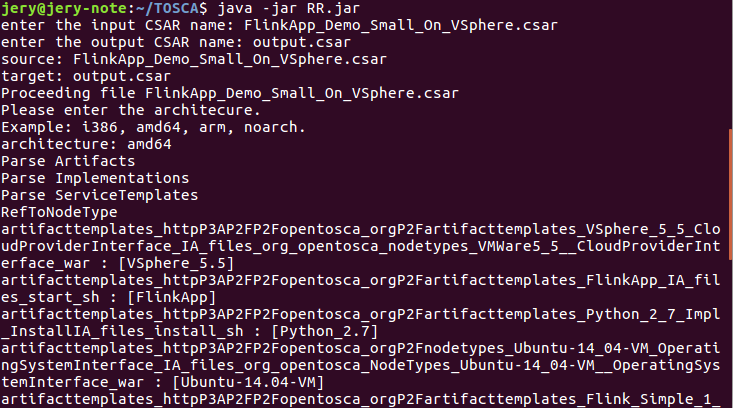
\includegraphics[width=0.7\textwidth]{Screenshot_processing}
%	\caption{Processing by the framework.}
%	\label{fig:process}
%\end{figure}
\section{Visualize with Winery}\label{sec:checkwin}
Winery was used to validate the correctness of the output CSARs. 
 This is a tool for the development of TOSCA systems and is useful for verify the results. %\\
 The input CSAR's representation by Winery is displayed in Figure~\ref{fig:winery_source2}.
 It contains external references but they are resolved by the framework and exchanged by new nodes in the output CSARs. 
 \begin{figure}[ht]   
 	\centering
 	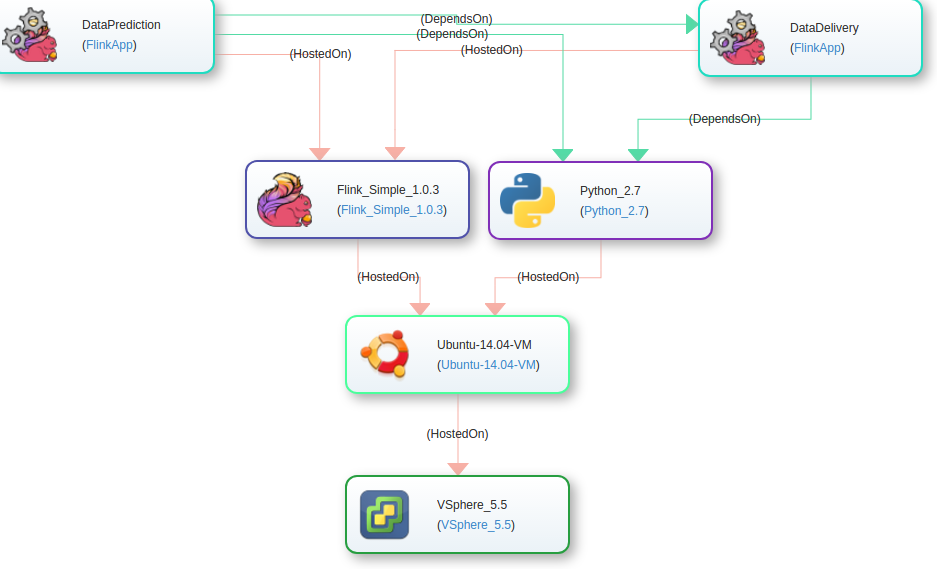
\includegraphics[width=0.7\textwidth]{Screenshot_winery_source2}
 	\caption{The input CSAR represented by $Winery$.\\\small http://www.opentosca.org/demos/smart-prediction-demo/index.html}
 	\label{fig:winery_source2}
 \end{figure}
   \\
 %\subsection*{Add to Winery}
 The output CSARs were added to Winery.
 Due to a significant increase in size of the first CSAR, this can be a fairly lengthy procedure.
Fully dependencies three for the Java package consists of about 60 packages and the python requires about 50 more. 
In the One node for one package mode for each of these packages a new node must be created.
It was only six nodes in the input CSAR, but after the processing, the first CSAR contains more than 100 of nodes.
This problem doesn't occur in the Sets of packages mode. 
For two external references only two additional nodes were created.
Therefore the addition of the second CSAR into Winery passes much faster. 
% Addition of a single node CSAR is faster process.
% The number of additional nodes coincides with the number of artifacts containing external references.
 During the addition, the syntax of the CSARs is tested.
 In a case of errors, messages will be displayed.
 \\
 %\subsection*{Display by Winery}
Then the CSARs were displayed.
To visualize a CSAR, Winery must validate and interpret it's internal references.
Due to the high number of nodes, the processing of the first CSAR lasts longer as the processing of the second CSAR. 
If something was defined not properly, these erroneous nodes or references between them will not be displayed.
The representation of the first CSAR is shown on Figure~\ref{fig:winery_output}, but only a part of the CSAR is visible.
The structure seems very difficult to follow.
An observer can identify four old nodes, two new nodes and a mix of references.
 To verify the topology some nodes was moved manually. 
 Figure~\ref{fig:winery_output2} displays the result. 
 Now its possible to identify references between some nodes.
The second CSAR with manually moved nodes is presented on Figure~\ref{fig:winery_output_single}, which shows the clear structure.
New nodes installing python and Java were created and referenced to nodes which contained external references earlier.\\
 The correctness of dependencies was verified by checking several references with the $apt$-$cache$ $depends$ command.
By opening the content of some nodes, it was verified, that there are right artifacts in new nodes and that external references were deleted from old nodes.
For example it was noted that the node installing python from the second CSAR contains more then 50 Deployment Artifacts and one Implementation Artifact which installs the corresponding packages.
 \begin{figure}[ht]   
 	\centering
 	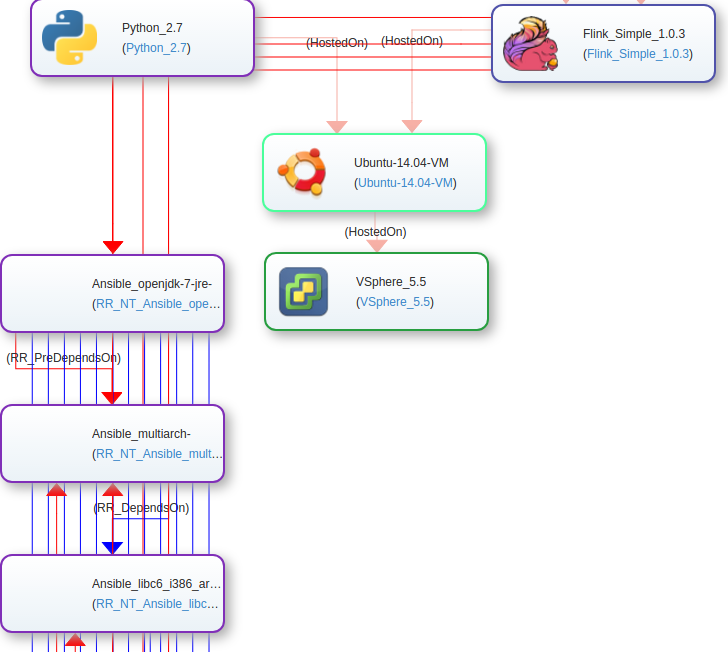
\includegraphics[width=0.7\textwidth]{Screenshot_winery_output}  
 	\caption{The CSAR processed in One node for one package mode and represented by Winery.}
 	\label{fig:winery_output}
 \end{figure}
 \begin{figure}[ht]   
 	\centering
 	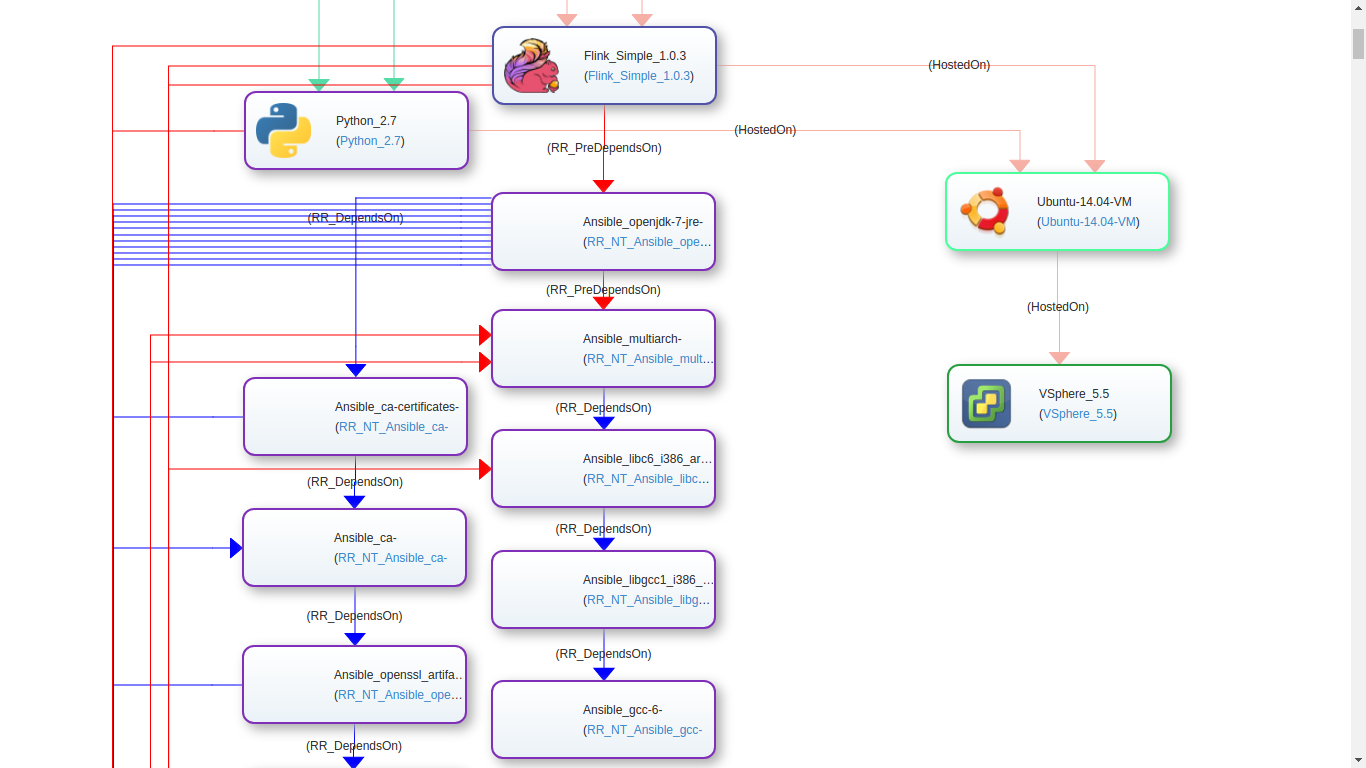
\includegraphics[width=0.7\textwidth]{Screenshot_winery_output2}
 	\caption{The CSAR processed in One node for one package mode and represented by Winery with some nodes moved manually.}
 	\label{fig:winery_output2}
 \end{figure}
\begin{figure}[ht]   
	\centering
	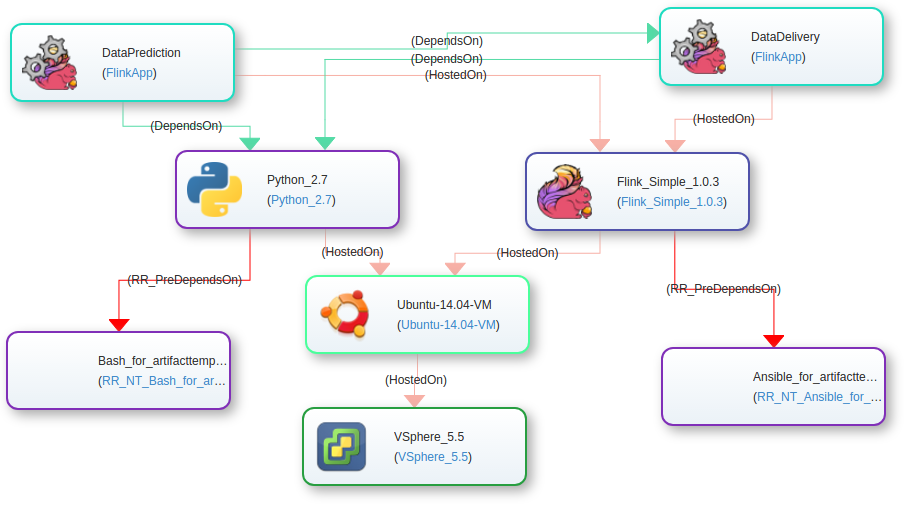
\includegraphics[width=0.7\textwidth]{Screenshot_winery_output_single}
	\caption{The representation of the CSAR processed in the Sets of packages mode.}
	\label{fig:winery_output_single}
\end{figure}
\section{Validate Artifacts}\label{sec:checkart}
It is necessary to verify whether it is possible to install new packages using the generated artifacts.
At first Bash scripts and then ansible playbooks will be tested.

\subsection*{Validate Bash Scripts}
Since Bash is used in the Linux's command line, it will be pretty easy to check Bash installation scripts by starting them.
Of course that must be done with the necessary privileges.
For the script file installing the $python2.7$-$minimal$ package, the command will be $sudo$ $RR\_python2\_7$-$minimal.sh$.
%An example of the $python2.7$ installation is presented in listing~\ref{lst:check_bash_script}. %\\
The installation ended without any warnings or errors, which means that it was completed successfully.
This way any generated Bash script can be validated.
%\begin{Listing}
%	\caption{Check Bash installation script}
%	\label{lst:check_bash_script}
%	\begin{lstlisting}
%	user@user:~$ sudo RR_python2_7-minimal.sh 
%	(Reading database ... 286091 files and directories currently installed.)
%	Preparing to unpack python2_7-minimal.deb ...
%	Unpacking python2.7-minimal (2.7.12-1ubuntu0~16.04.1) over (2.7.12-1ubuntu0~16.04.1) ...
%	Setting up python2.7-minimal (2.7.12-1ubuntu0~16.04.1) ...
%	Processing triggers for man-db (2.7.5-1) ...
%	\end{lstlisting}
%\end{Listing}

\subsection*{Validate Ansible Playbooks}
To validate an ansible playbook we need to extract the zip file containing the playbook manually. 
During the regular execution, this work will be done by a runtime environment.
The call to the ansible runtime which proceeds the playbook is a simple procedure too.
For the playbook with the $main$.$yml$ name, the command will be $sudo$ $ansible$-$playbook$ $main.yml$.
%An example is provided in Figure~\ref{fig:ansible_output2}. %\\
$Ok$ at the end of the output signals that the installation was completed successfully.
%\begin{figure}[ht]   
%	\centering
%	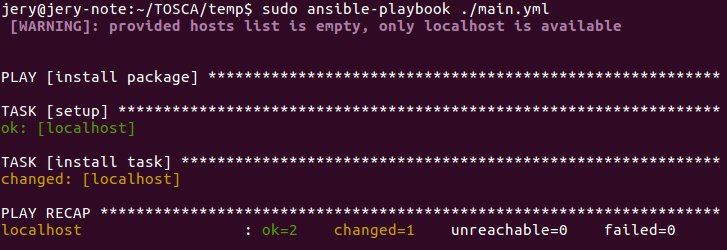
\includegraphics[width=0.7\textwidth]{Screenshot_ansible_output}
%	\caption{An ansible playbook's execution process}
%	\label{fig:ansible_output2}
%\end{figure}